\documentclass[letter,11pt]{article}
\usepackage{graphicx, csvsimple, pgfplotstable}
\usepackage{wrapfig}
\usepackage[letter, inner=2cm, outer=2cm, top=2cm, bottom=2cm, offset=0cm]{geometry}
\author{Kenneth Cross \\
        Math 177 \\
        San Jose State University}
\title{\textbf{Employee Schedule Optimization}}
\date{\today}

\begin{document}
\maketitle
\newpage

\section{The Problem}

The problem to be optimized is and employee schedule. 
More specifically, who might be the best people to schedule in a restaurant on any given day?
While this problem uses a restaurant as its main example, the solutions can be applied to any shift-based industry.
Since the problem stems from the availability of people, the solution is not obvious, other things must be performed before a \emph{integer linear optimization} model can be formed.

\section{The Solution}

First, we start by representing peoples availability in a matrix, showing which jobs they can perform and which days they can work.
Since there are variables that suggest it would be more beneficial for one person to work on a given day then another, they are attached as the last columns.
This gives us a matrix that can be optimized.
And the goal is to maximize the sum of the last few columns which will later be reorganized leaving $x_1 + x_2 + x_3$.
$x_1$ is whether this employee is a preferred employee, or rather, they earn more sales than others do.
$x_2$ is whether this employee is scheduled for a position they prefer.
$x_3$ is the consideration of the difficulty of the day.
If the day is difficult, then a skilled employee should be favored.

For each day of the week, there is a matrix like this, \\ 

\csvautotabular{../data/mathcpy.csv}
\\
Since multiple people may work the same shift, a separate matrix that shows shift scheduling demands is also used for further analysis and approximations. \\

\csvautotabular{../data/shift_class.csv}
\\
Instead of solving for combinatorial output of every person that can work together in a given day, an approximation is done, where there is something like a scan line performed.
It works by looking at all available shifts and people that can fill them, it assumes that each job can be filled by one person, then it will calculate the optimal solution for the people who can fill it and append the result to the corresponding columns until all the jobs are filled.

\section{Methodology}

1) Staff Generation: Stored in a possibility matrix \\
2) Staff Optimization \\ 
3) Schedule Based on Staff Optimization Sum \\ 
4) Schedule Satisfaction Optimization \\ 

\begin{figure}
    \includegraphics[width=18cm]{graph.eps}
    \caption{\small Algorithm Digraph}
\end{figure}

\section{Modules and Functions}

The entire depth of the inner workings of the program/algorithm are outlined here. 
The subsections try to follow a logical working order of pragmatic flow.

\subsection{Rostering Optimizations}

There are currently four values considered for the final roster optimizer value.
The day difficulty, outstanding employee, position preference, and the employee day preference values and their relationship are what determine the optimizer value.
Any undesirable relationships and traits are given zero points or subtract points, as optimizer values can be negative.
Day preferences are given on the availability grid with a value of zero through five, where zero indicates the impossibility of work and five is the most highly desired day to work.
The position preference value currently only determines the preference of one position, and it is a number, the position index to which they prefer.
The other two values are boolean, which is easy to sum.

All positive relationships and values are given one point and summed, except all the points on day preferences are added instead of a single point.

The relationships needed to accrue points are the following:
1) Outstanding employee and difficult day
2) Difficult day with no outstanding employee in preferred position, then a point is subtracted.

The entire roster is sorted from highest to lowest by optimizer value then given to the scheduler function.

\subsection{Multi-Shift Support}

This should be taken care of in the scheduler algorithm rather than the rostering algorithm.
This makes sense because rostering will calculate all possibilities of a person's availability rather than overlook other possibilities for other shifts.
The scheduler should have a section to combine and compare full shift schedules where logic should be performed for optimizations and shifting conflicts or other legal parameters.

\section{Data Representations}

Incoming input is currently contained in two separate CSV files. 
One file contains employee availability where the position section is a preference as to how many times per week someone would like to perform that position. The other file contains what types of positions are required and how many of each for every day of the week.
The CSV files are then read into python where they are stored as integer matrices.
All of the following operations are performed in python, but the actual program has not been written to completion.


\end{document}
